\documentclass[14pt, a0paper, portrait]{tikzposter}
\usepackage[utf8]{inputenc}
 
\title{Flowing, Fast and Slow}\author{A Study of Fast-Slow Dynamics in Nonlinear Evolution Equations }
\institute{Jonna, Kieran, Tom }
\date{14/12/2018}

%\institute{MIGSAA}
 
% \usepackage{graphicx}
% \usepackage{sidecap}
\usepackage{caption}
\captionsetup{%
    ,format=hang
    ,justification=raggedright
    ,singlelinecheck=false
    ,figureposition=right
    }
% \usepackage{sidecap}
\usepackage{blindtext}
\usepackage{comment}
\usepackage{amsmath}
\usepackage{graphicx}% http://ctan.org/pkg/graphicx
\usepackage{array}% http://ctan.org/pkg/array
%\usepackage{proj1}
% \usetheme{Board}
\usetheme{Envelope}
 \colorlet{blockbodybgcolor}{white!60}

\begin{document}
 
\maketitle
\begin{columns}
    \column{0.5}

\block{Definition: Fast-Slow System}
    {Fast-slow systems are systems of differential equations that can be viewed on two different time scales, which are separated by a parameter, $\epsilon$. The transition between those two systems is done by a transformation of the time variable, $t = \frac{\tau}{\epsilon}$. 
In this project two and three dimensional systems are considered.
The two dimensional problem is considered in detail, while the three dimensional case is only introduced briefly.
}
\block{The Van der Pol System}
{The dynamics of the 2-dimensional Van der Pol system is investigated in the following. The behaviour of the system depends on the behaviour of the parameter $\lambda$. The two representative values of $\lambda$, namely $\lambda =1$ and $\lambda = O(\sqrt{\epsilon})$ are analysed in parallel below.
We employ the strategy outlined above for $\lambda=1$, by investigating the flow of the Van der Pol in the limit $\epsilon \to 0$, find the fold points where hyperbolicity breaks down (highlighted in green on the phase portrait), and apply the Blow-Up method in order to analyse the dynamics for $\epsilon>0$, found in the singular limit.



}


\column{0.5}
\block{Aims and Strategy}
{
\begin{tabular}{p{0.9\linewidth}p{0.1\linewidth}}
{
The aim of the project is to understand the global dynamics of the fast-slow system. However, the system is non-linear and therefore not analytically solvable. 
In order to understand the dynamics, the following strategy is employed:
\begin{itemize}
    \item Consider the singular limit as $\epsilon\to 0$ and analyse its dynamics.
    \item Deduce that the dynamics exist for the full system from the dynamics in the singular limit. To do this:
    \begin{itemize}
        \item The singular system needs to be normally hyperbolic. However, this hyperbolicity is not present in singular points.
        % \item Problem: There exist singular points (folds) where hyperbolicity gets lost
        \item Treat the fold points by employing the Blow-up Method. 
        \item Gain enough hyperbolicity to conclude persistence of dynamics for $\epsilon >0$.
    \end{itemize}
\end{itemize}
}
&
{

}
\end{tabular}
}


\end{columns} 

\begin{columns}
    \column{0.5}
    \block{Van der Pol System, $\lambda=1$}
{
% \begin{tabular}[cc]{p{0.5\linewidth}p{0.5\linewidth}}
\begin{minipage}{0.5\linewidth}
\begin{align*}{
\text{Fast System}=
    \begin{cases} x'=y-\frac{x^3}{3}+x\\
    y'=\epsilon(-1+ x),
    \end{cases}
}&\\
&\notag\\
{
\text{Slow System}= 
    \begin{cases} \epsilon \dot{x}=y-\frac{x^3}{3}+x\\
    \dot{y}=-1+x,
    \end{cases}
}\end{align*}\end{minipage}
\begin{minipage}{0.50\linewidth}
% \end{tabular}
% \column{0.25}
	\begin{tikzfigure}
% 		\centering
% 		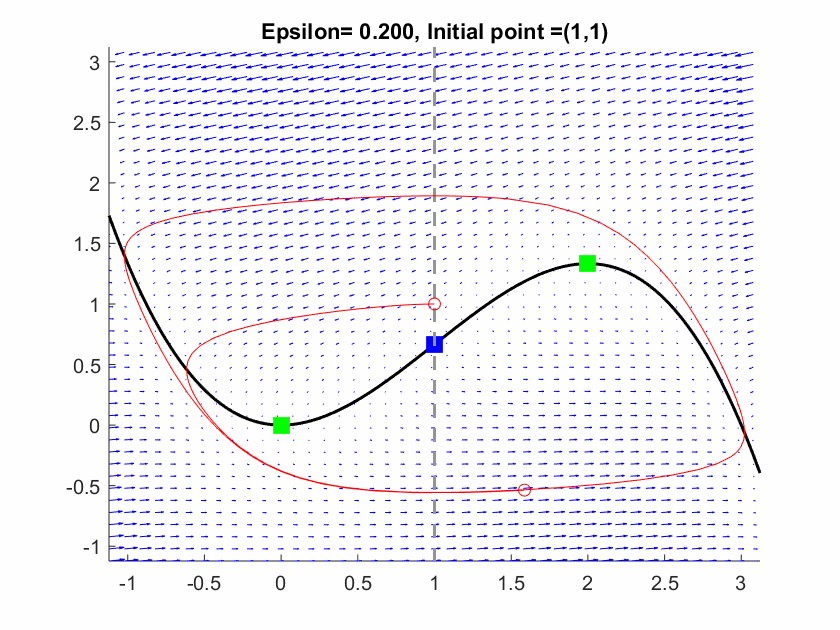
\includegraphics[height=8cm,width=10cm]{Posterpic1.jpg}
		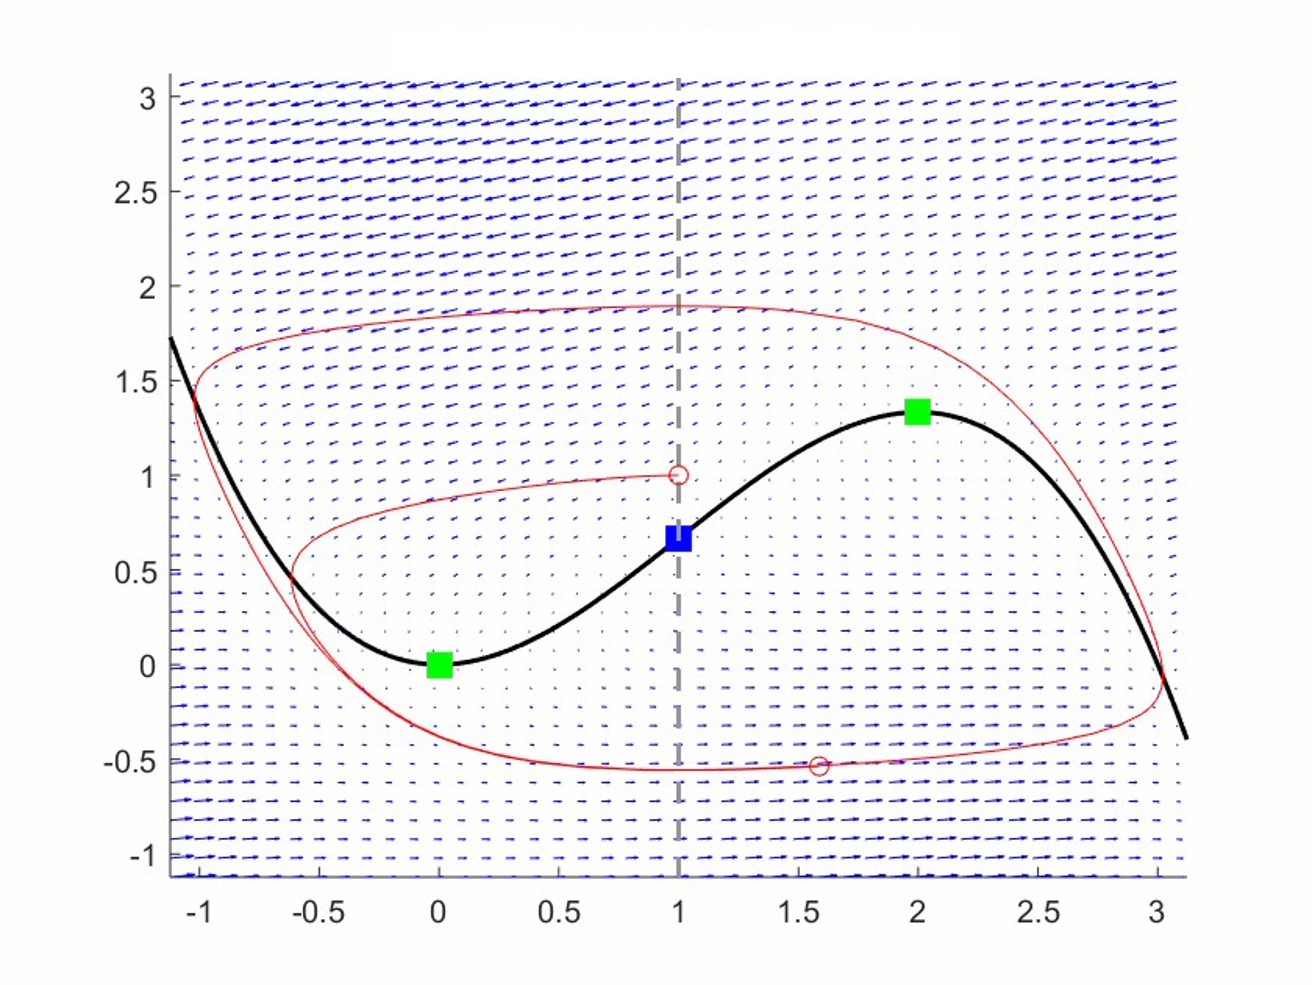
\includegraphics[height=8cm,width=10cm]{Images/vdPe02-Moment-big-e-pres.jpg}
		%\caption{Phase Portrait}
		%label{fig: Canard Point}
	\end{tikzfigure}
\end{minipage}
% \end{tabular}
% 	\begin{table}
% 	\begin{tabular}{c|c}
% 	     {  	\begin{tikzfigure}	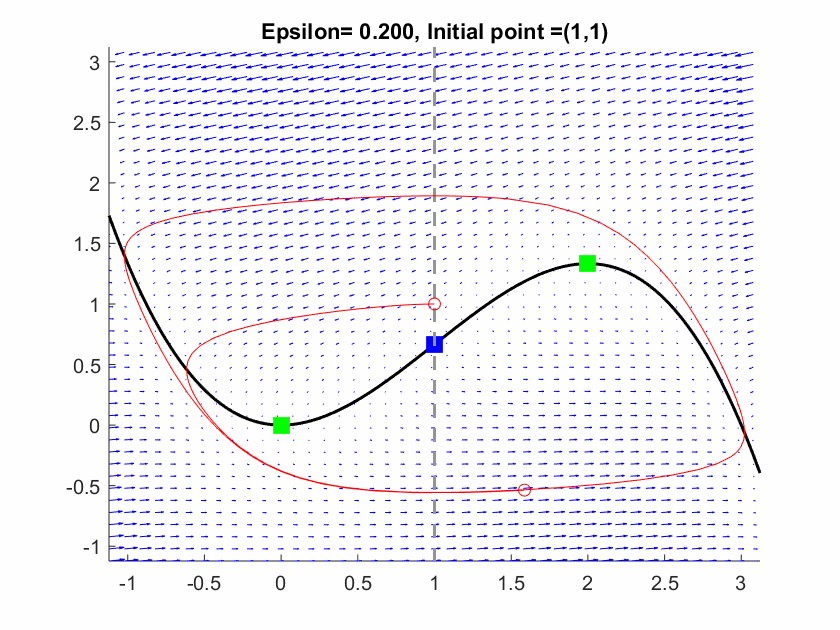
\includegraphics[height=8cm,width=10cm]{Posterpic1.jpg}
% \end{tikzfigure}    }
% 	     & {Phase Portrait}
% 	\end{tabular}
    % \end{table}
From this figure it is easy to see the trajectory of the flow jumping between from the repelling to attracting branches, where the green squares are the fold points. We also note that having a relatively large $\epsilon$ forces the flow to be further away from the fold point then our singular limits.}

\column{0.5}
\block{Van der Pol System, $\lambda= O(\sqrt{\epsilon})$}
{
% \begin{tabular}[cc]{p{0.5\linewidth}p{0.5\linewidth}}
\begin{minipage}{0.5\linewidth}
\begin{align*}{
\text{Fast System}=
    \begin{cases} x'=y-\frac{x^3}{3}+x\\
    y'=\epsilon(-\lambda+ x),
    \end{cases}
}&\\
&\notag\\
{
\text{Slow System}= 
    \begin{cases} \epsilon \dot{x}=y-\frac{x^3}{3}+x\\
    \dot{y}=-\lambda+x,
    \end{cases}
}\end{align*}\end{minipage}
\begin{minipage}{0.50\linewidth}
% \end{tabular}
% \column{0.25}
	\begin{tikzfigure}
% 		\centering
        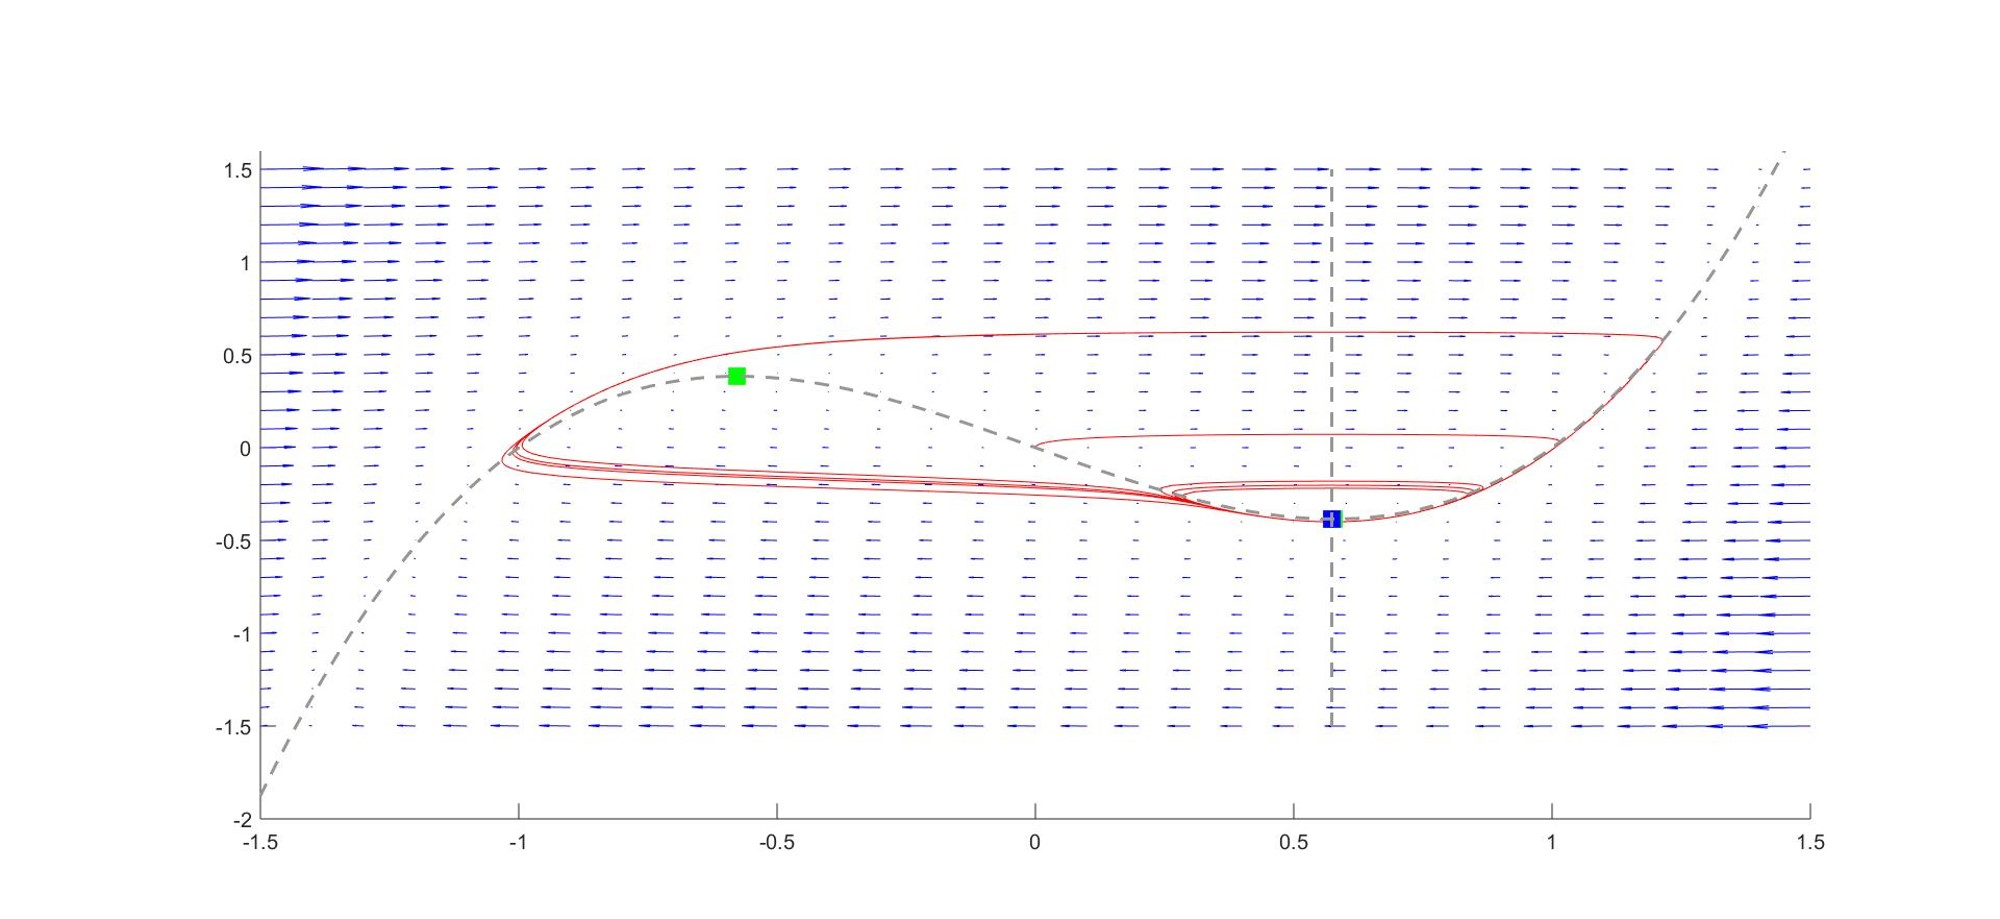
\includegraphics[height=8cm,width=10cm]{Code/behaviourswitch-pres.jpg}
		%\caption{Phase Portrait}
		%label{fig: Canard Point}
	\end{tikzfigure}
\end{minipage}

% \begin{minipage}{0.5\linewidth}
% % {\begin{tabular}{p{0.5\linewidth}p{0.5\linewidth}}
% \begin{align}{
% \text{Layer Problem}=
%     \begin{cases} x'=y-\frac{x^3}{3}+x,\\
% 	y'=0,
% 	\end{cases}
% }&\\
% &\\
% {
% \text{Reduced Problem}= 
%     \begin{cases} 0=y-\frac{x^3}{3}+x:=f,\\
% 	\dot{y}=-x.
% 	\end{cases}
% }\end{align}
% % \end{tabular}
% \end{minipage}

% \begin{minipage}{0.5\linewidth}
% \begin{tikzfigure}[Phase Portrait]
% 		\centering
% % 		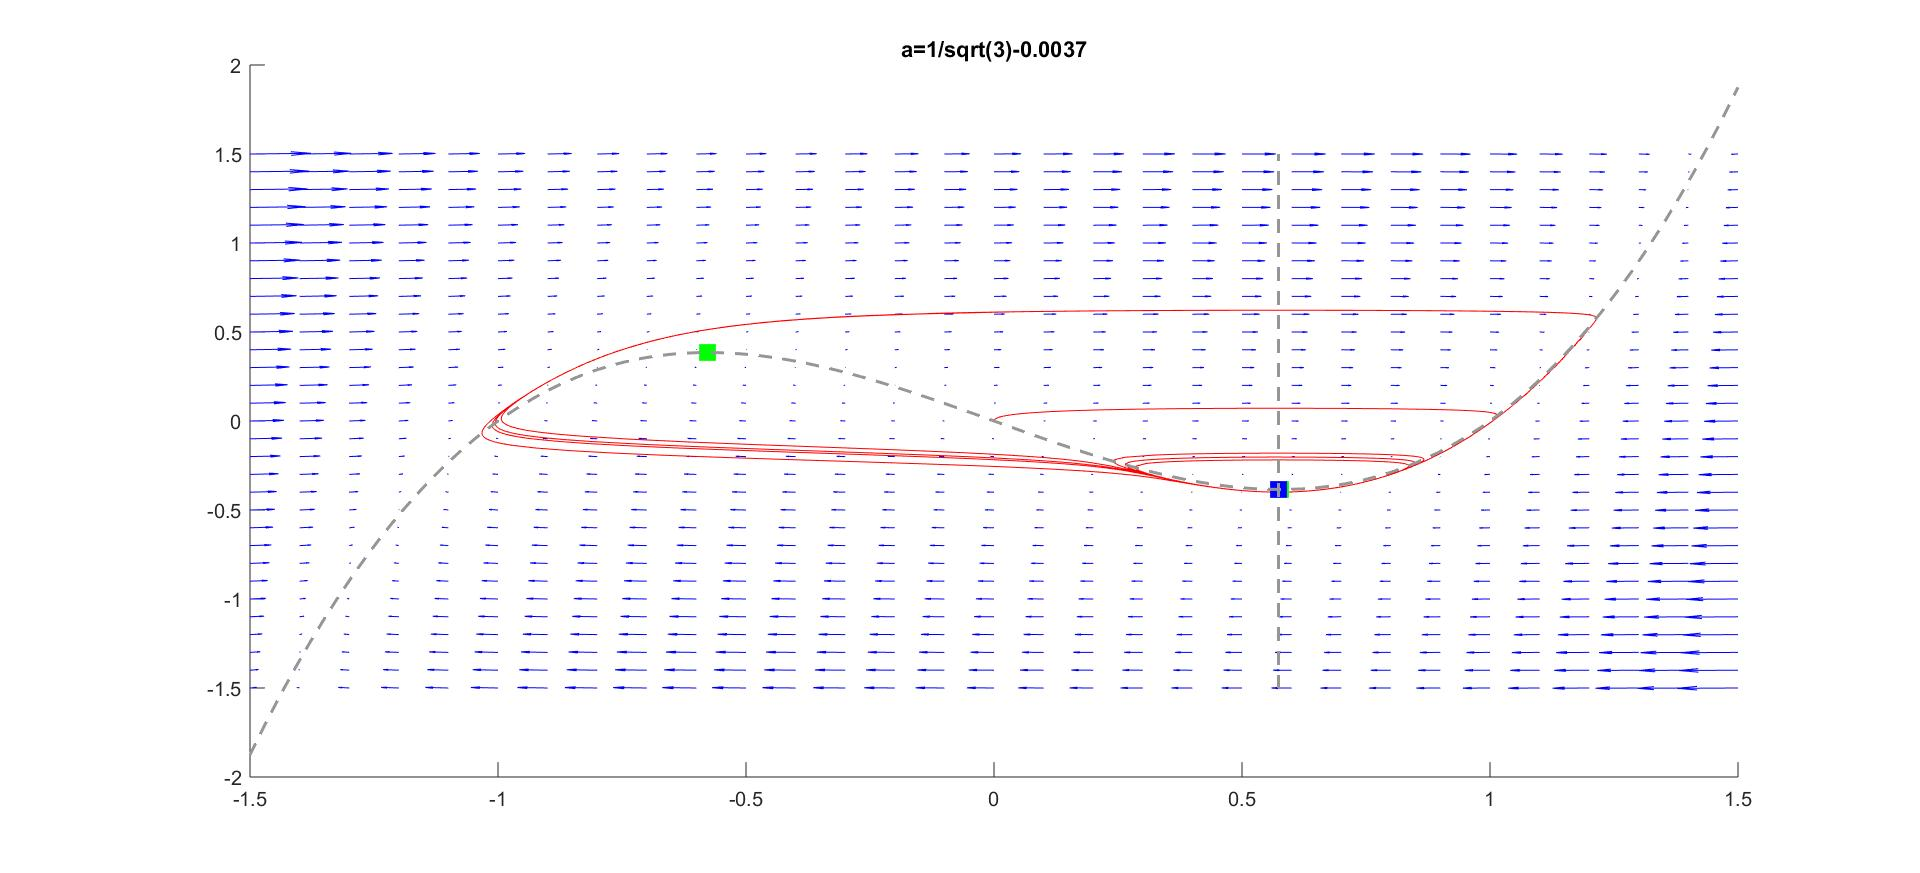
\includegraphics[height=8cm,width=10cm]{../Code/behaviourswitch}
% 		%\caption{The reduced flow where a) $\lambda=0$ and b) $\lambda>0$.}
% 		%label{fig: Canard Point}
% \end{tikzfigure}\end{minipage}
Now considering a general case when $\lambda>0$ we see that the canards exist where there are oscillations, near the fold point, and jumps at a distance $O(\sqrt{\epsilon})$ away from the fold, to another branch. If however, $\lambda$ is too large we find that the two connected branches will break which can lead to Hopf bifurcations and canard explosions, as seen here.}



\end{columns}
%%%%%%%%%%%%%%%%%%%%%%%%%%%%%%%%
%%%%%%%%%%%%%%%%%%%%%%%
%%%%%%%%%%%%%%
%%%%%%%%
\begin{columns}\column{0.5}
\block{Blow-Up Method}
{
    % \begin{tabular}{p{0.5\linewidth}p{0.1 \linewidth}p{0.2\linewidth}p{0.2\linewidth}}
    	For non-hyperbolic points we need to consider an alternative method of analysis - the Blow-Up Method. This, in essence, is a magnification of the non-hyperbolic fold point (green point on phase plane). To do this consider a coordinate transformation
    	\begin{align*}
    	x=\Bar{r}\Bar{x}, \        y=\Bar{r}^2\Bar{y}, \ \epsilon=\bar{r}^3\bar{\epsilon}.
    	\end{align*}
    	We then choose $\bar{y}=1, \ \bar{\epsilon}=1, \ \bar{x}=1$ respectively to analyse the flow in three different charts. These are expressed explicitly below. 
    	\begin{align*}
	& x=r_1x_1, y=r_1^2,  \epsilon=r_1^3\epsilon_1, \\%\label{sys: K1}\\
	& x=r_2x_2, \ y=r_2^2y_2, \epsilon=r_2^3, \\%\label{sys: K2}\\
	& x=r_3, \ y=r_3^2y_3,  \epsilon=r_3^3\epsilon_3% \label{sys:K3}
	\end{align*}

Substituting these transformations into the Van der Pol system above yields expressions for the flow in each of the three charts. }
    % 	& & 
\column{0.5}
\block{Charts}
%its working
{	\begin{minipage}{0.5\linewidth}

A convenient tool for the analysis of the blown up fold point is the use of charts.
We consider three charts to track the behaviour of a trajectory on different sections of the blown up fold point. For the canard case we only need to consider two charts, as the trajectory never flows through the region occupied by the third chart. The idea is to find the solution of the transformed equations in the individual charts and then use mapping transformations between the charts to follow a specific trajectory through each in order to create a global trajectory $\gamma$ that describes the full dynamics at the fold point. (This image is adapted from \cite{Kuehn})\end{minipage}	\begin{minipage}{0.5\linewidth}

\begin{tikzfigure}
    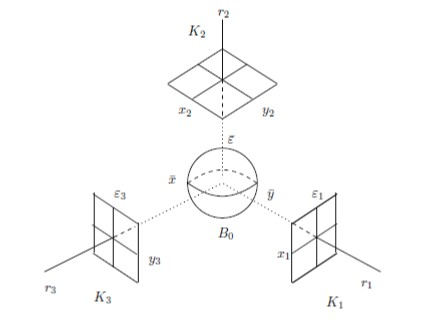
\includegraphics[height=5cm,width=6.5cm]{Images/charts-ball.jpg}
    % \caption
    \label{fig:my_label}
\end{tikzfigure}\end{minipage}

}
    % \end{tabular}
    
\end{columns}

\begin{columns}
\column{0.5}
\colorlet{blockbodybgcolor}{white!60}
\block{Global Solution when $\lambda=0$}
{
	\begin{minipage}{0.5\linewidth}

We find that the solution associated with the non-hyperbolic fold point is expressed by the above figure. The solution to the transformed system in chart two is known as the Riccati equations, and the global solution resembles this type of solution.
The analysis shows that the flow coming from $S^a$ is leaving the fold at $q_{out}$, which is equivalent to jumping off into the fast flow.
Studying the corresponding phase portrait, this is the expected dynamics.
For a small parameter regime $\lambda=O(\epsilon)$ the trajectory connects $S^a$ to $S^r$ instead of jumping off. (This image is adapted from \cite{krupa2001})\end{minipage}\begin{minipage}{0.5\linewidth}

	
	\begin{tikzfigure}
		\centering
		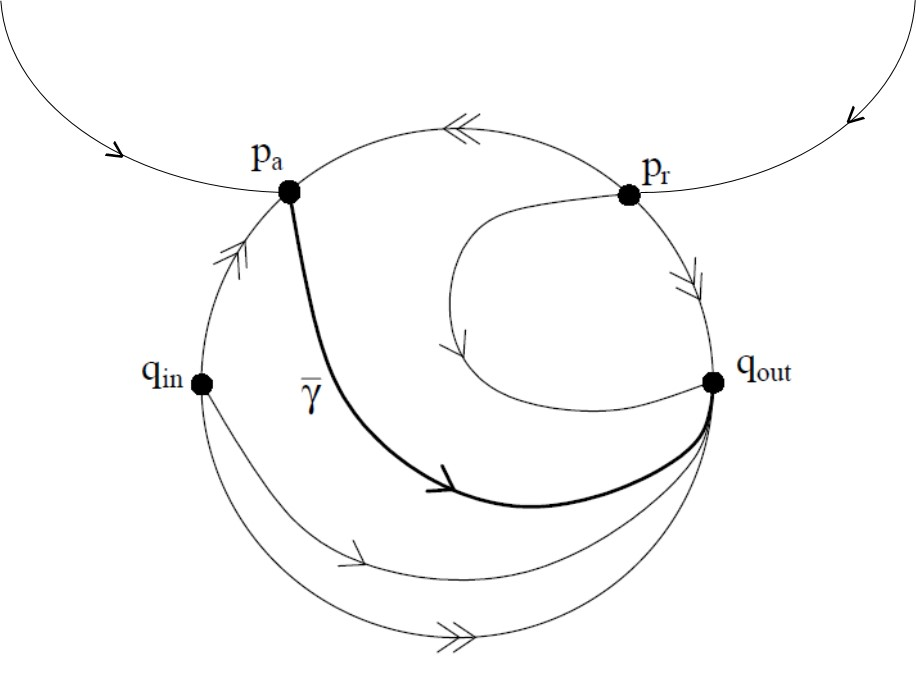
\includegraphics[height=8cm,width=10cm]{Poster/blow-up.jpg}
		%\caption{The reduced flow where a) $\lambda=0$ and b) $\lambda>0$.}
		%label{fig: Canard Point}
	\end{tikzfigure} \end{minipage}}


	\column{0.5}
   \block{Global Solution when $\lambda=O(\epsilon)$}
{	\begin{minipage}{0.5\linewidth}

	\begin{tikzfigure}
		\centering
		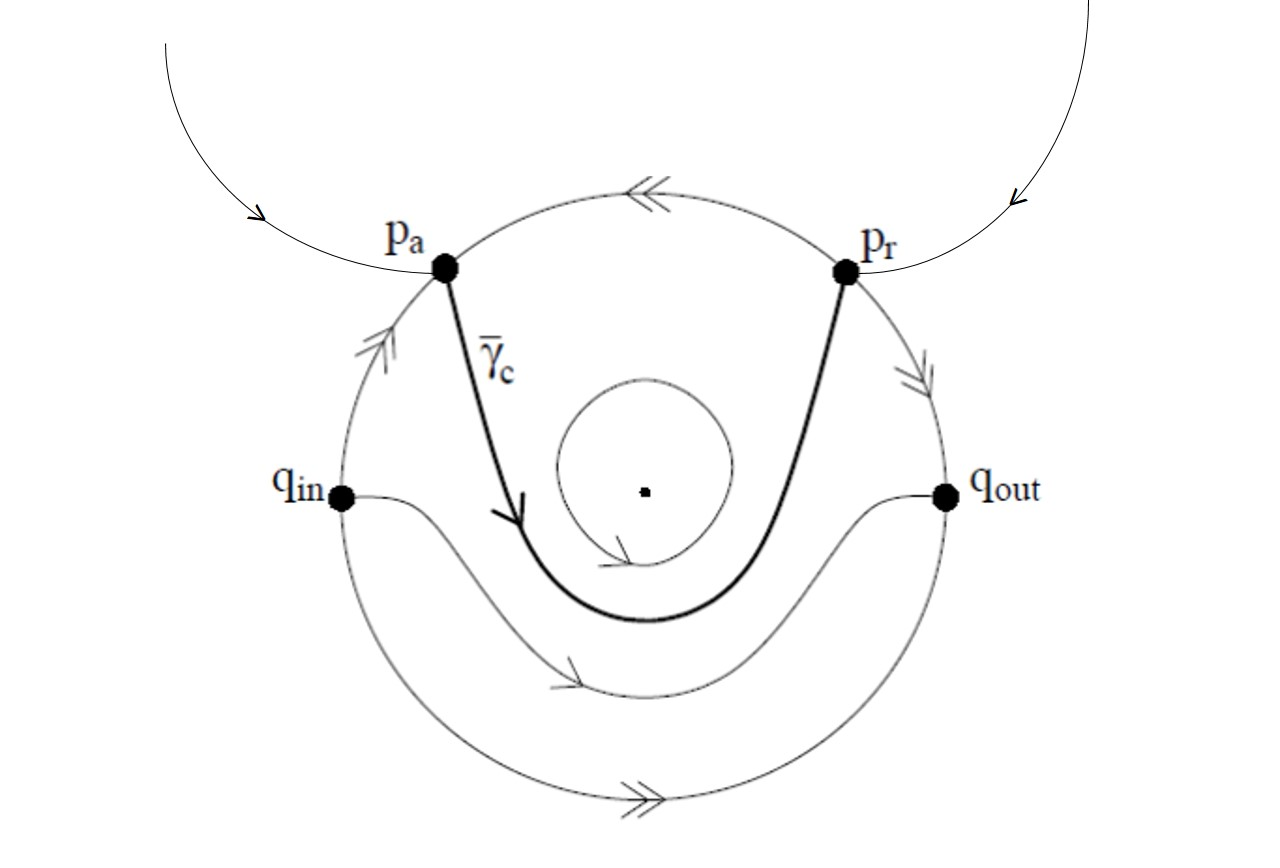
\includegraphics[height=8cm,width=10cm]{Images/pres-cancard.jpg}
		%\caption{The reduced flow where a) $\lambda=0$ and b) $\lambda>0$.}
		%label{fig: Canard Point}
    \end{tikzfigure}\end{minipage}	\begin{minipage}{0.5\linewidth}

    In the case when the trajectory $\gamma$ connects $p_a$ to $p_b$, it is called a canard. We expect different type of solutions exponentially close to the fold point. This is evident from the presence of a periodic solution above the canard solution $\gamma$. Below $\gamma$ we expect the solution to jump, as seen in the previous case. It is worth noting that the canard solutions only exist in an arbitrarily small region of $O(\sqrt{\epsilon})$. (This image is adapted from \cite{krupa2001})\end{minipage}}
\end{columns}


%%%%%%%%%%%%%%%%%%%%%%%%%%%%%%%%%%%%%%%%%%%%%%%%%%%%%%%%%%
%%%%%%%%%%%%%%%%%%%%%%%%%
%%%%%%%%%%%%%%


\block{Mixed-Mode Oscillations}
{	In the planar case, canards only occur within $O(\sqrt{\epsilon})$ of the fold point. To get more readily observable canards, another variable is introduced. This can lead to trajectories switching between large amplitude oscillations (LAO) and small amplitude oscillations (SAO). This is known as a mixed-mode oscillator.
	
	$$\begin{cases} \dot{x} = y-x^2-x^3\\ \dot{y} = \epsilon(z-x),\\ \dot{z}= \epsilon(-\nu-ax-by-cz)\\ \end{cases}$$
}
\begin{columns}
	\column{0.5}
	\colorlet{blockbodybgcolor}{white!60}
	\block{Folded Node Manifold}
	{ \begin{tikzfigure}
		\includegraphics[height=15cm,width=20cm]{Poster/foldNodeManifold.pdf}
	\end{tikzfigure}
	\centering{If we set $a=b=c=0$, the equilibrium is a node. The dynamics around the fold line in this case are shown in the image above (taken from \cite{MMO})}}
	
	
	
	\column{0.5}
	\block{MMO due to a Hopf Bifurcation}
	{Depending on the parameter values ($\nu,a,b,c$) more exotic behaviour can occur. For certain parameter regimes a chaotic trajectory is observed. However, these regimes are not well understood\\
	\begin{minipage}{0.5\linewidth}
		\begin{tikzfigure}
			\centering
			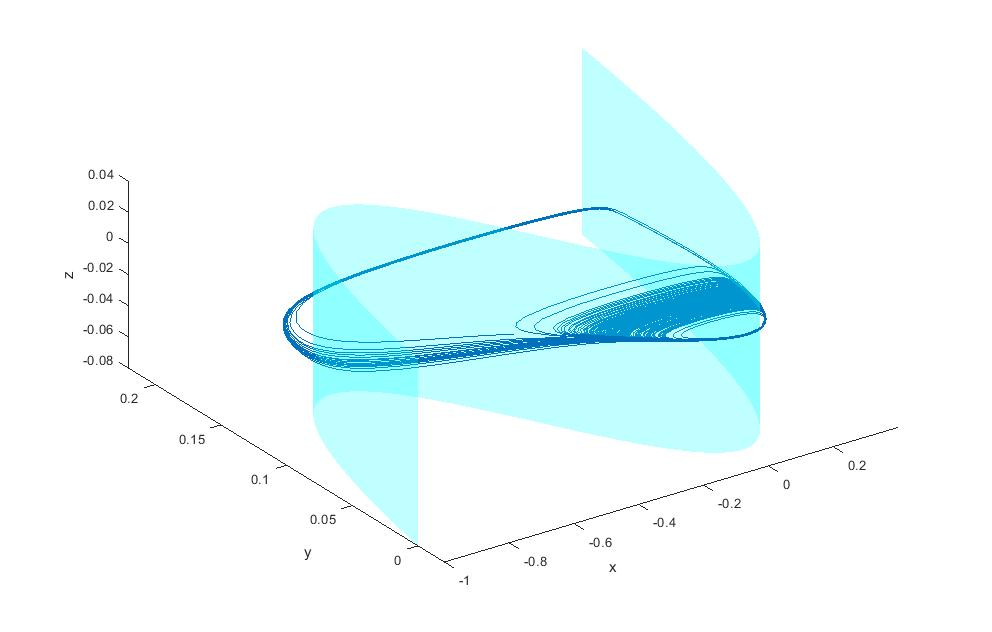
\includegraphics[height=15cm,width=20cm]{Poster/chaoticEvdp.jpg}
	\end{tikzfigure}
    \end{minipage}
    \begin{minipage}{0.50\linewidth}
	
	\begin{tikzfigure}
			\centering
			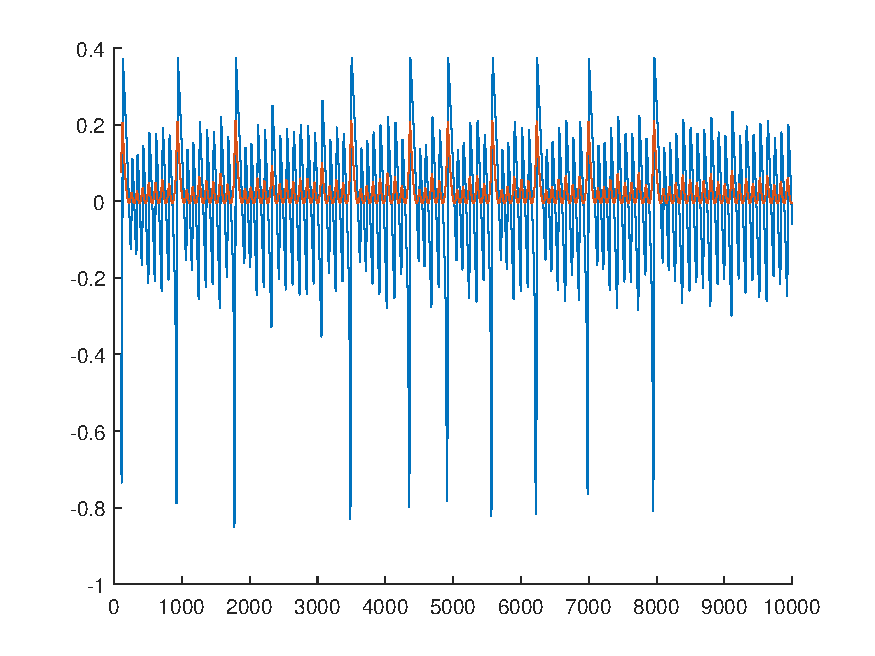
\includegraphics[height=15cm,width=18cm]{Poster/eVDPts.pdf}
	\end{tikzfigure}
\end{minipage}
}
\end{columns}

% (This image is taken from \citep{krupa2001})

\block{References}{

\begin{thebibliography}{1}
\bibliographystyle{abbrv}
\bibitem{krupa2001}Krupa, M. \& Szmolyan, P. (2001), `Extending geometric singular perturbation theory to nonhyperbolic points -- fold and canard points in two dimensions', SIAM J. Math. Analysis 33(2), 286--314.
\bibitem{MMO}Desroches, M., Guckenheimer, J., Krauskopf, B., Kuehn, C., Osinga, H. M. \& Wechselberger, M. (2012), `Mixed mode oscillations with multiple time scales', SIAM Rev. 54(2), 211-288

\bibitem{Kuehn} Kuehn, C. (2015), Multiple Time Scale Dynamics, Vol. 191 of Applied Mathematical Sciences, Springer International Publishing, Cham.
\end{thebibliography}
}


\end{document}